% Options for packages loaded elsewhere
\PassOptionsToPackage{unicode}{hyperref}
\PassOptionsToPackage{hyphens}{url}
%
\documentclass[
]{article}
\usepackage{amsmath,amssymb}
\usepackage{iftex}
\ifPDFTeX
  \usepackage[T1]{fontenc}
  \usepackage[utf8]{inputenc}
  \usepackage{textcomp} % provide euro and other symbols
\else % if luatex or xetex
  \usepackage{unicode-math} % this also loads fontspec
  \defaultfontfeatures{Scale=MatchLowercase}
  \defaultfontfeatures[\rmfamily]{Ligatures=TeX,Scale=1}
\fi
\usepackage{lmodern}
\ifPDFTeX\else
  % xetex/luatex font selection
\fi
% Use upquote if available, for straight quotes in verbatim environments
\IfFileExists{upquote.sty}{\usepackage{upquote}}{}
\IfFileExists{microtype.sty}{% use microtype if available
  \usepackage[]{microtype}
  \UseMicrotypeSet[protrusion]{basicmath} % disable protrusion for tt fonts
}{}
\makeatletter
\@ifundefined{KOMAClassName}{% if non-KOMA class
  \IfFileExists{parskip.sty}{%
    \usepackage{parskip}
  }{% else
    \setlength{\parindent}{0pt}
    \setlength{\parskip}{6pt plus 2pt minus 1pt}}
}{% if KOMA class
  \KOMAoptions{parskip=half}}
\makeatother
\usepackage{xcolor}
\usepackage[margin=1in]{geometry}
\usepackage{color}
\usepackage{fancyvrb}
\newcommand{\VerbBar}{|}
\newcommand{\VERB}{\Verb[commandchars=\\\{\}]}
\DefineVerbatimEnvironment{Highlighting}{Verbatim}{commandchars=\\\{\}}
% Add ',fontsize=\small' for more characters per line
\usepackage{framed}
\definecolor{shadecolor}{RGB}{248,248,248}
\newenvironment{Shaded}{\begin{snugshade}}{\end{snugshade}}
\newcommand{\AlertTok}[1]{\textcolor[rgb]{0.94,0.16,0.16}{#1}}
\newcommand{\AnnotationTok}[1]{\textcolor[rgb]{0.56,0.35,0.01}{\textbf{\textit{#1}}}}
\newcommand{\AttributeTok}[1]{\textcolor[rgb]{0.13,0.29,0.53}{#1}}
\newcommand{\BaseNTok}[1]{\textcolor[rgb]{0.00,0.00,0.81}{#1}}
\newcommand{\BuiltInTok}[1]{#1}
\newcommand{\CharTok}[1]{\textcolor[rgb]{0.31,0.60,0.02}{#1}}
\newcommand{\CommentTok}[1]{\textcolor[rgb]{0.56,0.35,0.01}{\textit{#1}}}
\newcommand{\CommentVarTok}[1]{\textcolor[rgb]{0.56,0.35,0.01}{\textbf{\textit{#1}}}}
\newcommand{\ConstantTok}[1]{\textcolor[rgb]{0.56,0.35,0.01}{#1}}
\newcommand{\ControlFlowTok}[1]{\textcolor[rgb]{0.13,0.29,0.53}{\textbf{#1}}}
\newcommand{\DataTypeTok}[1]{\textcolor[rgb]{0.13,0.29,0.53}{#1}}
\newcommand{\DecValTok}[1]{\textcolor[rgb]{0.00,0.00,0.81}{#1}}
\newcommand{\DocumentationTok}[1]{\textcolor[rgb]{0.56,0.35,0.01}{\textbf{\textit{#1}}}}
\newcommand{\ErrorTok}[1]{\textcolor[rgb]{0.64,0.00,0.00}{\textbf{#1}}}
\newcommand{\ExtensionTok}[1]{#1}
\newcommand{\FloatTok}[1]{\textcolor[rgb]{0.00,0.00,0.81}{#1}}
\newcommand{\FunctionTok}[1]{\textcolor[rgb]{0.13,0.29,0.53}{\textbf{#1}}}
\newcommand{\ImportTok}[1]{#1}
\newcommand{\InformationTok}[1]{\textcolor[rgb]{0.56,0.35,0.01}{\textbf{\textit{#1}}}}
\newcommand{\KeywordTok}[1]{\textcolor[rgb]{0.13,0.29,0.53}{\textbf{#1}}}
\newcommand{\NormalTok}[1]{#1}
\newcommand{\OperatorTok}[1]{\textcolor[rgb]{0.81,0.36,0.00}{\textbf{#1}}}
\newcommand{\OtherTok}[1]{\textcolor[rgb]{0.56,0.35,0.01}{#1}}
\newcommand{\PreprocessorTok}[1]{\textcolor[rgb]{0.56,0.35,0.01}{\textit{#1}}}
\newcommand{\RegionMarkerTok}[1]{#1}
\newcommand{\SpecialCharTok}[1]{\textcolor[rgb]{0.81,0.36,0.00}{\textbf{#1}}}
\newcommand{\SpecialStringTok}[1]{\textcolor[rgb]{0.31,0.60,0.02}{#1}}
\newcommand{\StringTok}[1]{\textcolor[rgb]{0.31,0.60,0.02}{#1}}
\newcommand{\VariableTok}[1]{\textcolor[rgb]{0.00,0.00,0.00}{#1}}
\newcommand{\VerbatimStringTok}[1]{\textcolor[rgb]{0.31,0.60,0.02}{#1}}
\newcommand{\WarningTok}[1]{\textcolor[rgb]{0.56,0.35,0.01}{\textbf{\textit{#1}}}}
\usepackage{graphicx}
\makeatletter
\def\maxwidth{\ifdim\Gin@nat@width>\linewidth\linewidth\else\Gin@nat@width\fi}
\def\maxheight{\ifdim\Gin@nat@height>\textheight\textheight\else\Gin@nat@height\fi}
\makeatother
% Scale images if necessary, so that they will not overflow the page
% margins by default, and it is still possible to overwrite the defaults
% using explicit options in \includegraphics[width, height, ...]{}
\setkeys{Gin}{width=\maxwidth,height=\maxheight,keepaspectratio}
% Set default figure placement to htbp
\makeatletter
\def\fps@figure{htbp}
\makeatother
\setlength{\emergencystretch}{3em} % prevent overfull lines
\providecommand{\tightlist}{%
  \setlength{\itemsep}{0pt}\setlength{\parskip}{0pt}}
\setcounter{secnumdepth}{-\maxdimen} % remove section numbering
\usepackage{booktabs}
\usepackage{longtable}
\usepackage{array}
\usepackage{multirow}
\usepackage{wrapfig}
\usepackage{float}
\usepackage{colortbl}
\usepackage{pdflscape}
\usepackage{tabu}
\usepackage{threeparttable}
\usepackage{threeparttablex}
\usepackage[normalem]{ulem}
\usepackage{makecell}
\usepackage{xcolor}
\ifLuaTeX
  \usepackage{selnolig}  % disable illegal ligatures
\fi
\usepackage{bookmark}
\IfFileExists{xurl.sty}{\usepackage{xurl}}{} % add URL line breaks if available
\urlstyle{same}
\hypersetup{
  pdftitle={Analisis Estadistico de Datos},
  pdfauthor={Grupo 05},
  hidelinks,
  pdfcreator={LaTeX via pandoc}}

\title{Analisis Estadistico de Datos}
\author{Grupo 05}
\date{2025-05-04}

\begin{document}
\maketitle

{
\setcounter{tocdepth}{2}
\tableofcontents
}
\begin{center}\rule{0.5\linewidth}{0.5pt}\end{center}

\section{Taller 02}\label{taller-02}

\textbf{Multivariada}\\
\textbf{Maestría en Energías Renovables}\\
\textbf{Escuela de Ingeniería, Ciencia y Tecnología}\\
\textbf{Universidad del Rosario}\\
\textbf{Integrantes:}\\
Zahira Itzel González Cleves\\
Diego Alejandro Mejía Montañez\\
Daniel Felipe Russi Aragón\\
Iván Camilo Granados Niño\\
Andrés Alfonso Osorio Marulanda

\begin{center}\rule{0.5\linewidth}{0.5pt}\end{center}

\section{Desarrollo Taller}\label{desarrollo-taller}

\begin{Shaded}
\begin{Highlighting}[]
\FunctionTok{library}\NormalTok{(corrplot)}
\FunctionTok{library}\NormalTok{(devtools)}
\FunctionTok{library}\NormalTok{(dplyr)}
\FunctionTok{library}\NormalTok{(factoextra)}
\FunctionTok{library}\NormalTok{(FactoMineR)}
\FunctionTok{library}\NormalTok{(ggExtra)}
\FunctionTok{library}\NormalTok{(GGally)}
\FunctionTok{library}\NormalTok{(ggplot2)}
\FunctionTok{library}\NormalTok{(kableExtra)}
\FunctionTok{library}\NormalTok{(knitr)}
\FunctionTok{library}\NormalTok{(MASS)}
\FunctionTok{library}\NormalTok{(plotly)}
\FunctionTok{library}\NormalTok{(psych)}
\FunctionTok{library}\NormalTok{(tidyverse)}
\FunctionTok{library}\NormalTok{(usethis)}
\FunctionTok{library}\NormalTok{(writexl)}

\CommentTok{\#carga de datos separados con sep=; }
\NormalTok{df\_pais }\OtherTok{\textless{}{-}} \FunctionTok{read.table}\NormalTok{(}\StringTok{"/Users/aosoriom/Repos/MER\_AEDatos/datasets/datos\_taller\_02.csv"}\NormalTok{,}\AttributeTok{sep=}\StringTok{";"}\NormalTok{,}\AttributeTok{header =} \ConstantTok{TRUE}\NormalTok{)}

\CommentTok{\# Visualiza la tabla de datos de mejor manera y con scroll}
\CommentTok{\# Para tablas pequeñas usar: kable(head(mi\_dataframe), caption = "Primeras filas del dataset")}
\FunctionTok{kable}\NormalTok{(}\FunctionTok{head}\NormalTok{(df\_pais), }\AttributeTok{caption =} \StringTok{"Primeras filas del dataset"}\NormalTok{) }\SpecialCharTok{\%\textgreater{}\%}
  \FunctionTok{scroll\_box}\NormalTok{(}\AttributeTok{width =} \StringTok{"100\%"}\NormalTok{, }\AttributeTok{height =} \StringTok{"auto"}\NormalTok{)}
\end{Highlighting}
\end{Shaded}

\begin{longtable}[t]{lrrrrrrrrrrrrrrrrrrrrrrrrrrrrrrrrrrrrrrrrrrrrrrrrrrrrrrrrr}
\caption{\label{tab:leer dataset}Primeras filas del dataset}\\
\toprule
Country & Bunker\_fuel\_consumption\_TBPD & Bunker\_residual\_fuel\_oil\_consumption\_TBPD & Crude\_oil\_including\_lease\_condensate\_exports\_TBPD & Crude\_oil\_including\_lease\_condensate\_imports\_TBPD & Crude\_oil\_including\_lease\_condensate\_production\_TBPD & Crude\_oil\_including\_lease\_condensate\_reserves\_BB & Distillate\_fuel\_oil\_consumption\_TBPD & Distillate\_fuel\_oil\_production\_TBPD & Jet\_fuel\_consumption\_TBPD & Jet\_fuel\_production\_TBPD & Kerosene\_consumption\_TBPD & Kerosene\_production\_TBPD & Liquefied\_petroleum\_gases\_.LPG.\_consumption\_TBPD & Liquefied\_petroleum\_gases\_.LPG.\_production\_TBPD & Motor\_gasoline\_consumption\_TBPD & Motor\_gasoline\_production\_TBPD & Natural\_gas\_plant\_liquids\_production\_TBPD & Other\_liquids\_production\_TBPD & Other\_refined\_products\_consumption\_TBPD & Other\_refined\_products\_production\_TBPD & Petroleum\_and\_other\_liquids\_CO2\_emissions\_MMTCD & Petroleum\_and\_other\_liquids\_consumption\_TBPD & Petroleum\_and\_other\_liquids\_production\_TBPD & Refined\_petroleum\_products\_consumption\_TBPD & Refined\_petroleum\_products\_production\_TBPD & Refinery\_processing\_gain\_TBPD & Residual\_fuel\_oil\_consumption\_TBPD & Residual\_fuel\_oil\_production\_TBPD & Biomass\_and\_waste\_electricity\_installed\_capacity\_MK & Biomass\_and\_waste\_electricity\_net\_generation\_BKWH & Electricity\_distribution\_losses\_BKWH & Electricity\_exports\_BKWH & Electricity\_imports\_BKWH & Electricity\_installed\_capacity\_MK & Electricity\_net\_consumption\_BKWH & Electricity\_net\_generation\_BKWH & Electricity\_net\_imports\_BKWH & Fossil\_fuels\_electricity\_installed\_capacity\_MK & Fossil\_fuels\_electricity\_net\_generation\_BKWH & Geothermal\_electricity\_installed\_capacity\_MK & Geothermal\_electricity\_net\_generation\_BKWH & Hydroelectric\_pumped\_storage\_electricity\_installed\_capacity\_MK & Hydroelectric\_pumped\_storage\_electricity\_net\_generation\_BKWH & Hydroelectricity\_installed\_capacity\_MK & Hydroelectricity\_net\_generation\_BKWH & Non.hydro\_renewable\_electricity\_installed\_capacity\_MK & Non.hydro\_renewable\_electricity\_net\_generation\_BKWH & Nuclear\_electricity\_installed\_capacity\_MK & Nuclear\_electricity\_net\_generation\_BKWH & Renewable\_electricity\_installed\_capacity\_MK & Renewable\_electricity\_net\_generation\_BKWH & Solar\_electricity\_installed\_capacity\_MK & Solar\_electricity\_net\_generation\_BKWH & Tide\_and\_wave\_electricity\_installed\_capacity\_MK & Tide\_and\_wave\_electricity\_net\_generation\_BKWH & Wind\_electricity\_installed\_capacity\_MK & Wind\_electricity\_net\_generation\_BKWH\\
\midrule
Albania & 0.6 & 0.0 & 19 & 0.9 & 21 & 0.2 & 16 & 1.8 & 0.2 & 0.0 & 0.0 & 0.0 & 3.9 & 0.0 & 2.8 & 0.0 & 0 & 0.0 & 5.4 & 4.7 & 3.7 & 28 & 21 & 28 & 6.6 & 0.0 & 0.1 & 0.1 & 0.0 & 0.0 & 2.8 & 0.2 & 3.3 & 1.8 & 5.0 & 4.7 & 3.1 & 0.1 & 0.0 & 0 & 0 & 0.0 & 0.0 & 1.7 & 4.7 & 0.0 & 0.0 & 0.0 & 0.0 & 1.7 & 4.7 & 0.0 & 0.0 & 0 & 0 & 0.0 & 0.0\\
Algeria & 14.0 & 3.8 & 581 & 6.4 & 1420 & 12.0 & 205 & 184.0 & 12.0 & 43.0 & 0.0 & 0.0 & 63.0 & 26.0 & 97.0 & 70.0 & 300 & 0.0 & 35.0 & 213.0 & 53.0 & 416 & 1722 & 416 & 658.0 & 1.8 & 4.0 & 120.0 & 0.0 & 0.0 & 11.0 & 0.9 & 0.7 & 16.0 & 49.0 & 60.0 & -0.2 & 16.0 & 60.0 & 0 & 0 & 0.0 & 0.0 & 0.3 & 0.3 & 0.0 & 0.0 & 0.0 & 0.0 & 0.3 & 0.3 & 0.0 & 0.0 & 0 & 0 & 0.0 & 0.0\\
Angola & 12.0 & 6.8 & 1632 & 0.0 & 1742 & 9.1 & 83 & 11.0 & 10.0 & 8.5 & 0.8 & 1.5 & 7.2 & 1.0 & 25.0 & 0.6 & 15 & 0.0 & 9.8 & 6.7 & 21.0 & 159 & 1756 & 159 & 47.0 & -0.7 & 23.0 & 17.0 & 0.0 & 0.0 & 1.1 & 0.0 & 0.0 & 1.8 & 8.1 & 9.2 & 0.0 & 0.8 & 4.2 & 0 & 0 & 0.0 & 0.0 & 1.0 & 5.0 & 0.0 & 0.0 & 0.0 & 0.0 & 1.0 & 5.0 & 0.0 & 0.0 & 0 & 0 & 0.0 & 0.0\\
Argentina & 48.0 & 26.0 & 49 & 9.5 & 532 & 2.8 & 232 & 173.0 & 33.0 & 29.0 & 0.5 & 0.3 & 56.0 & 39.0 & 122.0 & 123.0 & 104 & 65.0 & 221.0 & 204.0 & 101.0 & 764 & 713 & 764 & 661.0 & 12.0 & 99.0 & 93.0 & 0.2 & 1.0 & 18.0 & 0.2 & 10.0 & 38.0 & 123.0 & 131.0 & 9.9 & 25.0 & 92.0 & 0 & 0 & 1.0 & -0.2 & 10.0 & 32.0 & 0.5 & 1.6 & 1.6 & 5.3 & 11.0 & 34.0 & 0.0 & 0.0 & 0 & 0 & 0.2 & 0.6\\
Australia & 14.0 & 13.0 & 224 & 441.0 & 353 & 1.4 & 433 & 213.0 & 139.0 & 82.0 & 0.6 & 0.1 & 61.0 & 16.0 & 320.0 & 241.0 & 58 & 7.0 & 148.0 & 42.0 & 150.0 & 1126 & 442 & 1126 & 607.0 & 23.0 & 23.0 & 12.0 & 0.8 & 3.5 & 12.0 & 0.0 & 0.0 & 68.0 & 229.0 & 242.0 & 0.0 & 50.0 & 205.0 & 0 & 0 & 2.6 & 0.0 & 5.7 & 18.0 & 9.9 & 18.0 & 0.0 & 0.0 & 16.0 & 36.0 & 5.3 & 4.0 & 0 & 0 & 3.8 & 10.0\\
\addlinespace
Austria & 0.0 & 0.0 & 0 & 152.0 & 17 & 0.0 & 152 & 81.0 & 14.0 & 13.0 & 0.0 & 0.4 & 3.4 & 2.2 & 38.0 & 43.0 & 1 & 8.9 & 41.0 & 39.0 & 35.0 & 257 & 31 & 257 & 196.0 & 3.7 & 9.4 & 17.0 & 2.1 & 5.1 & 3.4 & 17.0 & 27.0 & 24.0 & 64.0 & 58.0 & 9.3 & 5.8 & 11.0 & 0 & 0 & 5.2 & -1.7 & 8.3 & 39.0 & 5.0 & 9.5 & 0.0 & 0.0 & 13.0 & 49.0 & 0.8 & 0.7 & 0 & 0 & 2.1 & 3.7\\
\bottomrule
\end{longtable}

\begin{Shaded}
\begin{Highlighting}[]
\CommentTok{\#summary(df\_pais)}
\end{Highlighting}
\end{Shaded}

\subsection{Normal Multivariada}\label{normal-multivariada}

\begin{center}\rule{0.5\linewidth}{0.5pt}\end{center}

\subsubsection{Pregunta 1}\label{pregunta-1}

\(w_1=5\)

Encuentre la estimación del vector de medias y la matriz de varianzas y
covarianzas para 5 variables de su interés del conjunto de datos.

\subsubsection{Vector de Medias}\label{vector-de-medias}

\begin{Shaded}
\begin{Highlighting}[]
\NormalTok{datos\_taller\_02 }\OtherTok{\textless{}{-}}\NormalTok{ df\_pais}
\CommentTok{\# Seleccionar las 5 variables de interés}
\NormalTok{vars\_interes }\OtherTok{\textless{}{-}}\NormalTok{ datos\_taller\_02[, }\FunctionTok{c}\NormalTok{(}\DecValTok{12}\NormalTok{, }\DecValTok{16}\NormalTok{, }\DecValTok{17}\NormalTok{, }\DecValTok{40}\NormalTok{, }\DecValTok{58}\NormalTok{)]}
\CommentTok{\# Estimación del vector de medias}
\NormalTok{vector\_medias }\OtherTok{\textless{}{-}} \FunctionTok{colMeans}\NormalTok{(vars\_interes)}
\FunctionTok{print}\NormalTok{(vector\_medias)}
\end{Highlighting}
\end{Shaded}

\begin{verbatim}
##                    Kerosene_consumption_TBPD 
##                                     8.224625 
##              Motor_gasoline_consumption_TBPD 
##                                   214.132432 
##               Motor_gasoline_production_TBPD 
##                                   211.467568 
## Fossil_fuels_electricity_net_generation_BKWH 
##                                   132.584084 
##         Wind_electricity_net_generation_BKWH 
##                                     6.084685
\end{verbatim}

Unidades en las que se miden las variables a estudiar: - TBPD (Thousand
Barrels Per Day) - BKWH (Billion Kilowatt-hours)

Se observa que el promedio de consumo de gasolina es muy alto en
comparación con otras variables, y que la generación eólica todavía es
baja en promedio.

\subsubsection{Matriz de varianzas y
covarianzas}\label{matriz-de-varianzas-y-covarianzas}

\begin{Shaded}
\begin{Highlighting}[]
\CommentTok{\# Estimación de la matriz de varianzas y covarianzas}
\NormalTok{matriz\_covarianzas }\OtherTok{\textless{}{-}} \FunctionTok{cov}\NormalTok{(vars\_interes)}
\FunctionTok{print}\NormalTok{(matriz\_covarianzas)}
\end{Highlighting}
\end{Shaded}

\begin{verbatim}
##                                              Kerosene_consumption_TBPD
## Kerosene_consumption_TBPD                                   1111.20579
## Motor_gasoline_consumption_TBPD                             3652.59338
## Motor_gasoline_production_TBPD                              4047.14314
## Fossil_fuels_electricity_net_generation_BKWH                4495.08919
## Wind_electricity_net_generation_BKWH                          91.56329
##                                              Motor_gasoline_consumption_TBPD
## Kerosene_consumption_TBPD                                           3652.593
## Motor_gasoline_consumption_TBPD                                   790595.046
## Motor_gasoline_production_TBPD                                    834206.418
## Fossil_fuels_electricity_net_generation_BKWH                      318100.939
## Wind_electricity_net_generation_BKWH                               18042.266
##                                              Motor_gasoline_production_TBPD
## Kerosene_consumption_TBPD                                          4047.143
## Motor_gasoline_consumption_TBPD                                  834206.418
## Motor_gasoline_production_TBPD                                   890035.397
## Fossil_fuels_electricity_net_generation_BKWH                     335168.583
## Wind_electricity_net_generation_BKWH                              19190.037
##                                              Fossil_fuels_electricity_net_generation_BKWH
## Kerosene_consumption_TBPD                                                        4495.089
## Motor_gasoline_consumption_TBPD                                                318100.939
## Motor_gasoline_production_TBPD                                                 335168.583
## Fossil_fuels_electricity_net_generation_BKWH                                   223824.714
## Wind_electricity_net_generation_BKWH                                            10183.494
##                                              Wind_electricity_net_generation_BKWH
## Kerosene_consumption_TBPD                                                91.56329
## Motor_gasoline_consumption_TBPD                                       18042.26614
## Motor_gasoline_production_TBPD                                        19190.03732
## Fossil_fuels_electricity_net_generation_BKWH                          10183.49430
## Wind_electricity_net_generation_BKWH                                    563.17167
\end{verbatim}

Las covarianzas (situadas fuera de la diagonal de la matriz) indican
cómo dos variables interactuan. Los valores positivos indican relación
directa o positiva, los valores negativos indican una relación indirecta
o negativa, es decir, mientra una aumenta la otra disminuye. Y por
último, si el valor es cero o cercano a cero, indica que las variables
no tienen relación.

Podemos concluir que:

\begin{itemize}
\item
  Motor\_gasoline\_consumption y production: Covarianza ≈ 834206.42 m
  Covarianza muy alta y positiva: los países que consumen más gasolina
  también tienden a producir más.
\item
  Kerosene y gasoline consumption: Covarianza ≈ 3652.59 Covarianza:
  positiva pero pequeña → Existe relación entre las variables, pero no
  muy fuerte.
\item
  Wind electricity vs.~cualquier otra: Covarianzas bajas (ej. con fósil
  ≈ 10183.49, con gasolina ≈ 18042.27), la generación eólica no tiene
  una fuerte relación lineal con las demás variables.
\end{itemize}

A continuación, se muestra la diagonal de la matriz de varianzas y
covarianzas, que representan la varianza de cada variable, es decir, qué
tanto se dispersan los datos respecto a su media.

\begin{Shaded}
\begin{Highlighting}[]
\CommentTok{\# Varianza de cada una de las variables}
\FunctionTok{print}\NormalTok{ (}\FunctionTok{diag}\NormalTok{(matriz\_covarianzas))}
\end{Highlighting}
\end{Shaded}

\begin{verbatim}
##                    Kerosene_consumption_TBPD 
##                                    1111.2058 
##              Motor_gasoline_consumption_TBPD 
##                                  790595.0460 
##               Motor_gasoline_production_TBPD 
##                                  890035.3975 
## Fossil_fuels_electricity_net_generation_BKWH 
##                                  223824.7141 
##         Wind_electricity_net_generation_BKWH 
##                                     563.1717
\end{verbatim}

\begin{itemize}
\item
  La producción y consumo de gasolina tienen altísima varianza, lo que
  sugiere grandes diferencias entre países.
\item
  La generación eólica tiene baja varianza, lo que indica que la mayoría
  de los países tienen valores similares (probablemente bajos).
\item
  La generación eléctrica por fósiles también muestra alta varianza, lo
  cual refleja diferencias estructurales entre países en sus sistemas
  eléctricos.
\end{itemize}

\subsection{ACP}\label{acp}

\begin{center}\rule{0.5\linewidth}{0.5pt}\end{center}

\subsubsection{Pregunta 2}\label{pregunta-2}

\(w_2=5\)

Realice un análisis descriptivo univariado y bivariado del conjunto de
datos. Considere nuevamente las mismas 5 variables de su interés para
este punto.

\subsubsection{Análisis univariado}\label{anuxe1lisis-univariado}

Resumen estadístico

\begin{Shaded}
\begin{Highlighting}[]
\FunctionTok{summary}\NormalTok{(vars\_interes)}
\end{Highlighting}
\end{Shaded}

\begin{verbatim}
##  Kerosene_consumption_TBPD Motor_gasoline_consumption_TBPD
##  Min.   :  0.000           Min.   :   0.8                 
##  1st Qu.:  0.000           1st Qu.:  13.0                 
##  Median :  0.500           Median :  33.0                 
##  Mean   :  8.225           Mean   : 214.1                 
##  3rd Qu.:  2.300           3rd Qu.: 108.5                 
##  Max.   :298.000           Max.   :8921.0                 
##  Motor_gasoline_production_TBPD Fossil_fuels_electricity_net_generation_BKWH
##  Min.   :   0.0                 Min.   :   0.00                             
##  1st Qu.:   5.6                 1st Qu.:   4.25                             
##  Median :  37.0                 Median :  21.00                             
##  Mean   : 211.5                 Mean   : 132.58                             
##  3rd Qu.: 106.5                 3rd Qu.:  80.00                             
##  Max.   :9571.0                 Max.   :3985.00                             
##  Wind_electricity_net_generation_BKWH
##  Min.   :  0.000                     
##  1st Qu.:  0.000                     
##  Median :  0.100                     
##  Mean   :  6.085                     
##  3rd Qu.:  1.450                     
##  Max.   :182.000
\end{verbatim}

Desviación estándar para cada variable

\begin{Shaded}
\begin{Highlighting}[]
\FunctionTok{sapply}\NormalTok{(vars\_interes, sd, }\AttributeTok{na.rm =} \ConstantTok{TRUE}\NormalTok{)}
\end{Highlighting}
\end{Shaded}

\begin{verbatim}
##                    Kerosene_consumption_TBPD 
##                                     33.33475 
##              Motor_gasoline_consumption_TBPD 
##                                    889.15412 
##               Motor_gasoline_production_TBPD 
##                                    943.41687 
## Fossil_fuels_electricity_net_generation_BKWH 
##                                    473.10117 
##         Wind_electricity_net_generation_BKWH 
##                                     23.73124
\end{verbatim}

\paragraph{Histograma de distribución para cada
variable}\label{histograma-de-distribuciuxf3n-para-cada-variable}

Histograma de distribución Kerosene\_consumption\_TBPD

\begin{Shaded}
\begin{Highlighting}[]
\FunctionTok{ggplot}\NormalTok{(vars\_interes, }\FunctionTok{aes}\NormalTok{(}\AttributeTok{x =}\NormalTok{ Kerosene\_consumption\_TBPD)) }\SpecialCharTok{+}
  \FunctionTok{geom\_histogram}\NormalTok{(}\AttributeTok{fill =} \StringTok{"steelblue"}\NormalTok{, }\AttributeTok{color =} \StringTok{"white"}\NormalTok{, }\AttributeTok{bins =} \DecValTok{50}\NormalTok{) }\SpecialCharTok{+}
  \FunctionTok{labs}\NormalTok{(}\AttributeTok{title =} \StringTok{"Distribución de Kerosene\_consumption\_TBPD"}\NormalTok{,}
       \AttributeTok{x =} \StringTok{"Consumo (TBPD)"}\NormalTok{,}
       \AttributeTok{y =} \StringTok{"Frecuencia"}\NormalTok{)}
\end{Highlighting}
\end{Shaded}

\includegraphics{T02_AEDatos_files/figure-latex/unnamed-chunk-1-1.pdf}
Histograma de distribución Motor\_gasoline\_consumption\_TBPD

\begin{Shaded}
\begin{Highlighting}[]
\FunctionTok{ggplot}\NormalTok{(vars\_interes, }\FunctionTok{aes}\NormalTok{(}\AttributeTok{x =}\NormalTok{ Motor\_gasoline\_consumption\_TBPD)) }\SpecialCharTok{+}
  \FunctionTok{geom\_histogram}\NormalTok{(}\AttributeTok{fill =} \StringTok{"steelblue"}\NormalTok{, }\AttributeTok{color =} \StringTok{"white"}\NormalTok{, }\AttributeTok{bins =} \DecValTok{50}\NormalTok{) }\SpecialCharTok{+}
  \FunctionTok{labs}\NormalTok{(}\AttributeTok{title =} \StringTok{"Distribución de Motor\_gasoline\_consumption\_TBPD"}\NormalTok{,}
       \AttributeTok{x =} \StringTok{"Consumo (TBPD)"}\NormalTok{,}
       \AttributeTok{y =} \StringTok{"Frecuencia"}\NormalTok{)}
\end{Highlighting}
\end{Shaded}

\includegraphics{T02_AEDatos_files/figure-latex/unnamed-chunk-2-1.pdf}

Histograma de distribución Motor\_gasoline\_production\_TBPD

\begin{Shaded}
\begin{Highlighting}[]
\FunctionTok{ggplot}\NormalTok{(vars\_interes, }\FunctionTok{aes}\NormalTok{(}\AttributeTok{x =}\NormalTok{ Motor\_gasoline\_production\_TBPD)) }\SpecialCharTok{+}
  \FunctionTok{geom\_histogram}\NormalTok{(}\AttributeTok{fill =} \StringTok{"steelblue"}\NormalTok{, }\AttributeTok{color =} \StringTok{"white"}\NormalTok{, }\AttributeTok{bins =} \DecValTok{50}\NormalTok{) }\SpecialCharTok{+}
  \FunctionTok{labs}\NormalTok{(}\AttributeTok{title =} \StringTok{"Distribución de Motor\_gasoline\_production\_TBPD"}\NormalTok{,}
       \AttributeTok{x =} \StringTok{"Consumo (TBPD)"}\NormalTok{,}
       \AttributeTok{y =} \StringTok{"Frecuencia"}\NormalTok{)}
\end{Highlighting}
\end{Shaded}

\includegraphics{T02_AEDatos_files/figure-latex/unnamed-chunk-3-1.pdf}

Histograma de distribución
Fossil\_fuels\_electricity\_net\_generation\_BKWH

\begin{Shaded}
\begin{Highlighting}[]
\FunctionTok{ggplot}\NormalTok{(vars\_interes, }\FunctionTok{aes}\NormalTok{(}\AttributeTok{x =}\NormalTok{ Fossil\_fuels\_electricity\_net\_generation\_BKWH)) }\SpecialCharTok{+}
  \FunctionTok{geom\_histogram}\NormalTok{(}\AttributeTok{fill =} \StringTok{"steelblue"}\NormalTok{, }\AttributeTok{color =} \StringTok{"white"}\NormalTok{, }\AttributeTok{bins =} \DecValTok{50}\NormalTok{) }\SpecialCharTok{+}
  \FunctionTok{labs}\NormalTok{(}\AttributeTok{title =} \StringTok{"Distribución de Fossil\_fuels\_electricity\_net\_generation\_BKWH"}\NormalTok{,}
       \AttributeTok{x =} \StringTok{"Consumo (BKWH)"}\NormalTok{,}
       \AttributeTok{y =} \StringTok{"Frecuencia"}\NormalTok{)}
\end{Highlighting}
\end{Shaded}

\includegraphics{T02_AEDatos_files/figure-latex/unnamed-chunk-4-1.pdf}

Histograma de distribución
Fossil\_fuels\_electricity\_net\_generation\_BKWH

\begin{Shaded}
\begin{Highlighting}[]
\FunctionTok{ggplot}\NormalTok{(vars\_interes, }\FunctionTok{aes}\NormalTok{(}\AttributeTok{x =}\NormalTok{ Wind\_electricity\_net\_generation\_BKWH)) }\SpecialCharTok{+}
  \FunctionTok{geom\_histogram}\NormalTok{(}\AttributeTok{fill =} \StringTok{"steelblue"}\NormalTok{, }\AttributeTok{color =} \StringTok{"white"}\NormalTok{, }\AttributeTok{bins =} \DecValTok{50}\NormalTok{) }\SpecialCharTok{+}
  \FunctionTok{labs}\NormalTok{(}\AttributeTok{title =} \StringTok{"Distribución de Wind\_electricity\_net\_generation\_BKWH"}\NormalTok{,}
       \AttributeTok{x =} \StringTok{"Consumo (BKWH)"}\NormalTok{,}
       \AttributeTok{y =} \StringTok{"Frecuencia"}\NormalTok{)}
\end{Highlighting}
\end{Shaded}

\includegraphics{T02_AEDatos_files/figure-latex/unnamed-chunk-5-1.pdf}
\#\#\#\# Boxplots Boxplot Kerosene\_consumption\_TBPD

\begin{Shaded}
\begin{Highlighting}[]
\FunctionTok{boxplot}\NormalTok{(vars\_interes}\SpecialCharTok{$}\NormalTok{Kerosene\_consumption\_TBPD)}
\end{Highlighting}
\end{Shaded}

\includegraphics{T02_AEDatos_files/figure-latex/unnamed-chunk-6-1.pdf}

Boxplot Motor\_gasoline\_consumption\_TBPD

\begin{Shaded}
\begin{Highlighting}[]
\FunctionTok{boxplot}\NormalTok{(vars\_interes}\SpecialCharTok{$}\NormalTok{Motor\_gasoline\_consumption\_TBPD)}
\end{Highlighting}
\end{Shaded}

\includegraphics{T02_AEDatos_files/figure-latex/unnamed-chunk-7-1.pdf}

Boxplot Motor\_gasoline\_production\_TBPD

\begin{Shaded}
\begin{Highlighting}[]
\FunctionTok{boxplot}\NormalTok{(vars\_interes}\SpecialCharTok{$}\NormalTok{Motor\_gasoline\_production\_TBPD)}
\end{Highlighting}
\end{Shaded}

\includegraphics{T02_AEDatos_files/figure-latex/unnamed-chunk-8-1.pdf}

Boxplot Fossil\_fuels\_electricity\_net\_generation\_BKWH

\begin{Shaded}
\begin{Highlighting}[]
\FunctionTok{boxplot}\NormalTok{(vars\_interes}\SpecialCharTok{$}\NormalTok{Fossil\_fuels\_electricity\_net\_generation\_BKWH)}
\end{Highlighting}
\end{Shaded}

\includegraphics{T02_AEDatos_files/figure-latex/unnamed-chunk-9-1.pdf}

Boxplot Wind\_electricity\_net\_generation\_BKWH

\begin{Shaded}
\begin{Highlighting}[]
\FunctionTok{boxplot}\NormalTok{(vars\_interes}\SpecialCharTok{$}\NormalTok{Wind\_electricity\_net\_generation\_BKWH)}
\end{Highlighting}
\end{Shaded}

\includegraphics{T02_AEDatos_files/figure-latex/unnamed-chunk-10-1.pdf}

\subsubsection{Análisis multivariado}\label{anuxe1lisis-multivariado}

La matriz de correlación indica la fuerza y dirección de las relaciones
lineales entre las variables de un conjunto de datos.

\begin{Shaded}
\begin{Highlighting}[]
\NormalTok{correlaciones }\OtherTok{\textless{}{-}} \FunctionTok{cor}\NormalTok{(vars\_interes, }\AttributeTok{use =} \StringTok{"complete.obs"}\NormalTok{)}
\FunctionTok{print}\NormalTok{(correlaciones)}
\end{Highlighting}
\end{Shaded}

\begin{verbatim}
##                                              Kerosene_consumption_TBPD
## Kerosene_consumption_TBPD                                    1.0000000
## Motor_gasoline_consumption_TBPD                              0.1232330
## Motor_gasoline_production_TBPD                               0.1286909
## Fossil_fuels_electricity_net_generation_BKWH                 0.2850277
## Wind_electricity_net_generation_BKWH                         0.1157454
##                                              Motor_gasoline_consumption_TBPD
## Kerosene_consumption_TBPD                                          0.1232330
## Motor_gasoline_consumption_TBPD                                    1.0000000
## Motor_gasoline_production_TBPD                                     0.9944726
## Fossil_fuels_electricity_net_generation_BKWH                       0.7561952
## Wind_electricity_net_generation_BKWH                               0.8550542
##                                              Motor_gasoline_production_TBPD
## Kerosene_consumption_TBPD                                         0.1286909
## Motor_gasoline_consumption_TBPD                                   0.9944726
## Motor_gasoline_production_TBPD                                    1.0000000
## Fossil_fuels_electricity_net_generation_BKWH                      0.7509407
## Wind_electricity_net_generation_BKWH                              0.8571400
##                                              Fossil_fuels_electricity_net_generation_BKWH
## Kerosene_consumption_TBPD                                                       0.2850277
## Motor_gasoline_consumption_TBPD                                                 0.7561952
## Motor_gasoline_production_TBPD                                                  0.7509407
## Fossil_fuels_electricity_net_generation_BKWH                                    1.0000000
## Wind_electricity_net_generation_BKWH                                            0.9070316
##                                              Wind_electricity_net_generation_BKWH
## Kerosene_consumption_TBPD                                               0.1157454
## Motor_gasoline_consumption_TBPD                                         0.8550542
## Motor_gasoline_production_TBPD                                          0.8571400
## Fossil_fuels_electricity_net_generation_BKWH                            0.9070316
## Wind_electricity_net_generation_BKWH                                    1.0000000
\end{verbatim}

\begin{itemize}
\item
  Alta correlación entre Motor\_gasoline\_consumption\_TBPD y
  Motor\_gasoline\_production\_TBPD: 0.9945. Esto indica una relación
  casi perfecta. Los países que más gasolina producen también la
  consumen mucho.
\item
  Alta correlación entre entre
  Fossil\_fuels\_electricity\_net\_generation\_BKWH y
  Wind\_electricity\_net\_generation\_BKWH: 0.9070. Los países que
  generan más electricidad con fósiles también tienen alta generación
  eólica.
\item
  Correlación fuerte entre Motor\_gasoline\_production\_TBPD y
  Wind\_electricity\_net\_generation\_BKWH: 0.8571. Los paises con alta
  producción de gasolina, también tienen una alta generación neta de
  electricidad eólica.
\item
  Kerosene\_consumption\_TBPD tiene correlaciones débiles con todas las
  demás (\textless{} 0.29).
\end{itemize}

\begin{Shaded}
\begin{Highlighting}[]
\FunctionTok{ggpairs}\NormalTok{(vars\_interes)}
\end{Highlighting}
\end{Shaded}

\includegraphics{T02_AEDatos_files/figure-latex/unnamed-chunk-12-1.pdf}
La mayoría de las variables tienen distribuciones sesgadas hacia valores
bajos con algunos valores muy altos (ver diagramas de dispersión).

Esto sugiere que la mayoría de los países tienen baja producción o
consumo, mientras que unos pocos tienen valores extremos.

\subsubsection{Pregunta 3}\label{pregunta-3}

\(w_3=8\)\\
El conjunto de datos incluye 57 variables, analizarlas de forma
individual podría representar un gasto computacional y de tiempo
bastante agotador; por lo cuál una técnica de reducción de
dimensionalidad sería ideal. Ejecute un ACP sobre estos datos, compare
la contribución de las variables sobre el primer plano factorial de un
ACP normado (escalado) y uno sin normalizar (sin escalar).

El conjunto de datos incluye 57 variables, analizarlas de forma
individual podría representar un gasto computacional y de tiempo
bastante agotador; por lo cual una técnica de reducción de
dimensionalidad sería ideal. Ejecute un ACP sobre estos datos, compare
la contribución de las variables sobre el primer plano factorial de un
ACP normado (escalado) y uno sin normalizar (sin escalar).

\begin{Shaded}
\begin{Highlighting}[]
\CommentTok{\#carga de datos separados con sep=; }
\NormalTok{pais }\OtherTok{=} \FunctionTok{read.table}\NormalTok{(}\StringTok{"/Users/aosoriom/Repos/MER\_AEDatos/datasets/datos\_taller\_02.csv"}\NormalTok{,}\AttributeTok{sep=}\StringTok{";"}\NormalTok{,}\AttributeTok{header =} \ConstantTok{TRUE}\NormalTok{)}

\CommentTok{\#se crea el data frame país }
\NormalTok{datos}\OtherTok{\textless{}{-}}\FunctionTok{as.data.frame}\NormalTok{(pais) }

\CommentTok{\#nueva variable y se le quita la 1ra columna }
\NormalTok{columnas\_a\_convertir }\OtherTok{\textless{}{-}} \FunctionTok{names}\NormalTok{(datos)[}\SpecialCharTok{{-}}\DecValTok{1}\NormalTok{] }

\CommentTok{\#transformación de datos a numéricos str(Datos)}
\NormalTok{datos[columnas\_a\_convertir] }\OtherTok{\textless{}{-}} \FunctionTok{lapply}\NormalTok{(datos[columnas\_a\_convertir], as.numeric)}
\CommentTok{\# str(datos) {-}{-}\textgreater{} se comenta para no sacar todos los datos, se debe quitar.}

\CommentTok{\#selección de las 5 variables}
\NormalTok{select\_data }\OtherTok{\textless{}{-}}\NormalTok{ datos[, }\FunctionTok{c}\NormalTok{(}\StringTok{"Refined\_petroleum\_products\_consumption\_TBPD"}\NormalTok{, }\StringTok{"Refined\_petroleum\_products\_production\_TBPD"}\NormalTok{, }\StringTok{"Electricity\_exports\_BKWH"}\NormalTok{, }\StringTok{"Electricity\_imports\_BKWH"}\NormalTok{, }\StringTok{"Electricity\_installed\_capacity\_MK"}\NormalTok{)]}
\FunctionTok{summary}\NormalTok{(select\_data)}
\end{Highlighting}
\end{Shaded}

\begin{verbatim}
##  Refined_petroleum_products_consumption_TBPD
##  Min.   :   15.0                            
##  1st Qu.:   71.5                            
##  Median :  202.0                            
##  Mean   :  811.4                            
##  3rd Qu.:  750.0                            
##  Max.   :19100.0                            
##  Refined_petroleum_products_production_TBPD Electricity_exports_BKWH
##  Min.   :    0.0                            Min.   : 0.000          
##  1st Qu.:   39.5                            1st Qu.: 0.000          
##  Median :  172.0                            Median : 0.600          
##  Mean   :  777.3                            Mean   : 5.158          
##  3rd Qu.:  555.0                            3rd Qu.: 5.550          
##  Max.   :19653.0                            Max.   :75.000          
##  Electricity_imports_BKWH Electricity_installed_capacity_MK
##  Min.   : 0.000           Min.   :   0.40                  
##  1st Qu.: 0.000           1st Qu.:   3.50                  
##  Median : 0.700           Median :  11.00                  
##  Mean   : 5.671           Mean   :  51.63                  
##  3rd Qu.: 7.550           3rd Qu.:  33.00                  
##  Max.   :67.000           Max.   :1380.00
\end{verbatim}

\begin{Shaded}
\begin{Highlighting}[]
\CommentTok{\#se excluye la primera columna}
\NormalTok{columnas\_numericas }\OtherTok{\textless{}{-}} \FunctionTok{names}\NormalTok{(datos)[}\SpecialCharTok{{-}}\DecValTok{1}\NormalTok{]}
 
\CommentTok{\#se aplica pca a datos normalizados o escalados}
 
\CommentTok{\#"prcom()p" es la forma rápida de implementar un PCA sobre un conjunto de datos, es necesaria la biblioteca stats, center y SCALE TRUE corresponden a las medias y desv estándar antes de aplicar el PCA}
\NormalTok{pca\_normalizado }\OtherTok{\textless{}{-}} \FunctionTok{prcomp}\NormalTok{(datos[, columnas\_numericas], }\AttributeTok{center =} \ConstantTok{TRUE}\NormalTok{, }\AttributeTok{scale =} \ConstantTok{TRUE}\NormalTok{)}
 
\CommentTok{\#se aplica pca a datos sin normalizar}
\NormalTok{pca\_sin\_normalizar }\OtherTok{\textless{}{-}} \FunctionTok{prcomp}\NormalTok{(datos[, columnas\_numericas], }\AttributeTok{center =} \ConstantTok{FALSE}\NormalTok{, }\AttributeTok{scale =} \ConstantTok{FALSE}\NormalTok{)}
 
\CommentTok{\#se comparan las contirbuciones de las variables seleccionadas}
\NormalTok{contribucion\_normalizado }\OtherTok{\textless{}{-}}\NormalTok{ pca\_normalizado}\SpecialCharTok{$}\NormalTok{sdev}\SpecialCharTok{\^{}}\DecValTok{2}
\NormalTok{contribucion\_sin\_normalizar }\OtherTok{\textless{}{-}}\NormalTok{ pca\_sin\_normalizar}\SpecialCharTok{$}\NormalTok{sdev}\SpecialCharTok{\^{}}\DecValTok{2}
 
\CommentTok{\#creación de tabla de datos para luego ver las contribuciones}
\NormalTok{contribuciones\_df }\OtherTok{\textless{}{-}} \FunctionTok{data.frame}\NormalTok{(}
  \AttributeTok{Contribucion\_Normalizado =}\NormalTok{ contribucion\_normalizado,}
  \AttributeTok{Contribucion\_Sin\_Normalizar =}\NormalTok{ contribucion\_sin\_normalizar)}
\CommentTok{\#print(format(contribuciones\_df, scientific=FALSE))}
\FunctionTok{head}\NormalTok{(contribuciones\_df, }\AttributeTok{n=}\DecValTok{10}\NormalTok{)}
\end{Highlighting}
\end{Shaded}

\begin{verbatim}
##    Contribucion_Normalizado Contribucion_Sin_Normalizar
## 1                35.3158793                27524045.470
## 2                 4.4099873                 4204746.774
## 3                 3.9984709                  470085.023
## 4                 2.7056000                  134152.350
## 5                 2.4548859                  109320.329
## 6                 1.8678717                   42942.129
## 7                 1.3074352                   22302.380
## 8                 1.1151341                   13868.073
## 9                 0.9019626                   12746.905
## 10                0.7565284                    9601.909
\end{verbatim}

Con las variables seleccionadas que presentan valores bajos con respecto
a otros países se observa que las contribuciones tienen poca influencia
en la variación de los datos después de ser normalizados, por lo que se
puede decir que dichas variables no contribuyen con aportes
significativos al primer componente principal con datos escalados. Para
los datos sin normalizar, las contribuciones son mayores comparadas con
las normalizadas debido a los rangos o escalas de las variables
seleccionadas no normalizadas.

\subsubsection{Pregunta 4}\label{pregunta-4}

\(w_4=8\)\\
Una vez calculado el PCA normado, ¿qué número de componentes principales
deberíamos seleccionar? ¿Bajo que criterio seleccionó este número de
componentes?

Se toma como referencia dos criterios 1) el Criterio de Kaiser que
define que se deben conservar o seleccionar aquellos cuyos valores
propios son iguales o superiores a 1 y 2) Porcentaje de la varianza
acumulada, en el cual se calcula el porcentaje de la varianza de cada
componente y se realiza el calculo del acumulado con el aporte de cada
componente hasta que se evidencia un valor significativo de este
porcentaje acumulado.

\begin{enumerate}
\def\labelenumi{\arabic{enumi})}
\item
  Criterio Kaiser: se selecciona hasta el componente principal 8, el
  cual es \(PC_1=1.11\) y cumple son ser mayor que 1. En otras palabras,
  se seleccionana del componente 1 al 8 por ser mayores a 1.
\item
  Criterio de \% de Varianza acumulada:usualmente se toman los
  componentes principales que totalicen una varianza acumulada entre
  70\% y 90\%. Para este ejercicio se usara el principio de Pareto
  identificando los componentes que alcancen una varianza acumulada
  igual o superior al 80\%, los cuales serian de los componentes del 1
  al 4; estos 4 componentes equivalen al 7\% del total y representan el
  81.8\% de la varianza acumulada.
\end{enumerate}

\subsubsection{Pregunta 5}\label{pregunta-5}

\(w_5=8\)\\
Analice la representación de las variables originales sobre las dos
primeras componentes en el primer plano factorial. ¿Que conclusiones
podemos sacar de este análisis?

En el siguiente diagrama fasorial se grafican los 2 componentes
principales, la misma es un poco difusa porque se están graficando las
57 variables.

\begin{Shaded}
\begin{Highlighting}[]
\CommentTok{\#agrupa los datos por componentes principales escalados y los guarda en la variable asignada acp\_c (para reducir el tamaño del nombre de las variables se utiliza IA)}
\CommentTok{\# La sintaxis [, {-}1] selecciona todas las filas (espacio antes de la coma)}
\CommentTok{\# y todas las columnas excepto la columna en el índice 1 (el {-}1 después de la coma)}
\NormalTok{datos\_rec }\OtherTok{\textless{}{-}} \FunctionTok{read.table}\NormalTok{(}\StringTok{"/Users/aosoriom/Repos/MER\_AEDatos/datasets/datos\_taller\_02\_rec.csv"}\NormalTok{,}\AttributeTok{sep=}\StringTok{";"}\NormalTok{,}\AttributeTok{header =} \ConstantTok{TRUE}\NormalTok{)}
\NormalTok{datos\_solo\_numericos }\OtherTok{\textless{}{-}}\NormalTok{ datos\_rec[, }\SpecialCharTok{{-}}\DecValTok{1}\NormalTok{]}
\NormalTok{acp\_c }\OtherTok{\textless{}{-}}\FunctionTok{prcomp}\NormalTok{(datos\_solo\_numericos, }\AttributeTok{scale =} \ConstantTok{TRUE}\NormalTok{)}

\FunctionTok{fviz\_pca\_var}\NormalTok{(acp\_c,}\AttributeTok{axes=}\FunctionTok{c}\NormalTok{(}\DecValTok{1}\NormalTok{,}\DecValTok{2}\NormalTok{),}\AttributeTok{repel=}\ConstantTok{TRUE}\NormalTok{, }\AttributeTok{labelsize=}\DecValTok{3}\NormalTok{, }\AttributeTok{arrowsize=}\FloatTok{0.5}\NormalTok{, }\AttributeTok{arrowwidth=}\FloatTok{0.5}\NormalTok{)}
\end{Highlighting}
\end{Shaded}

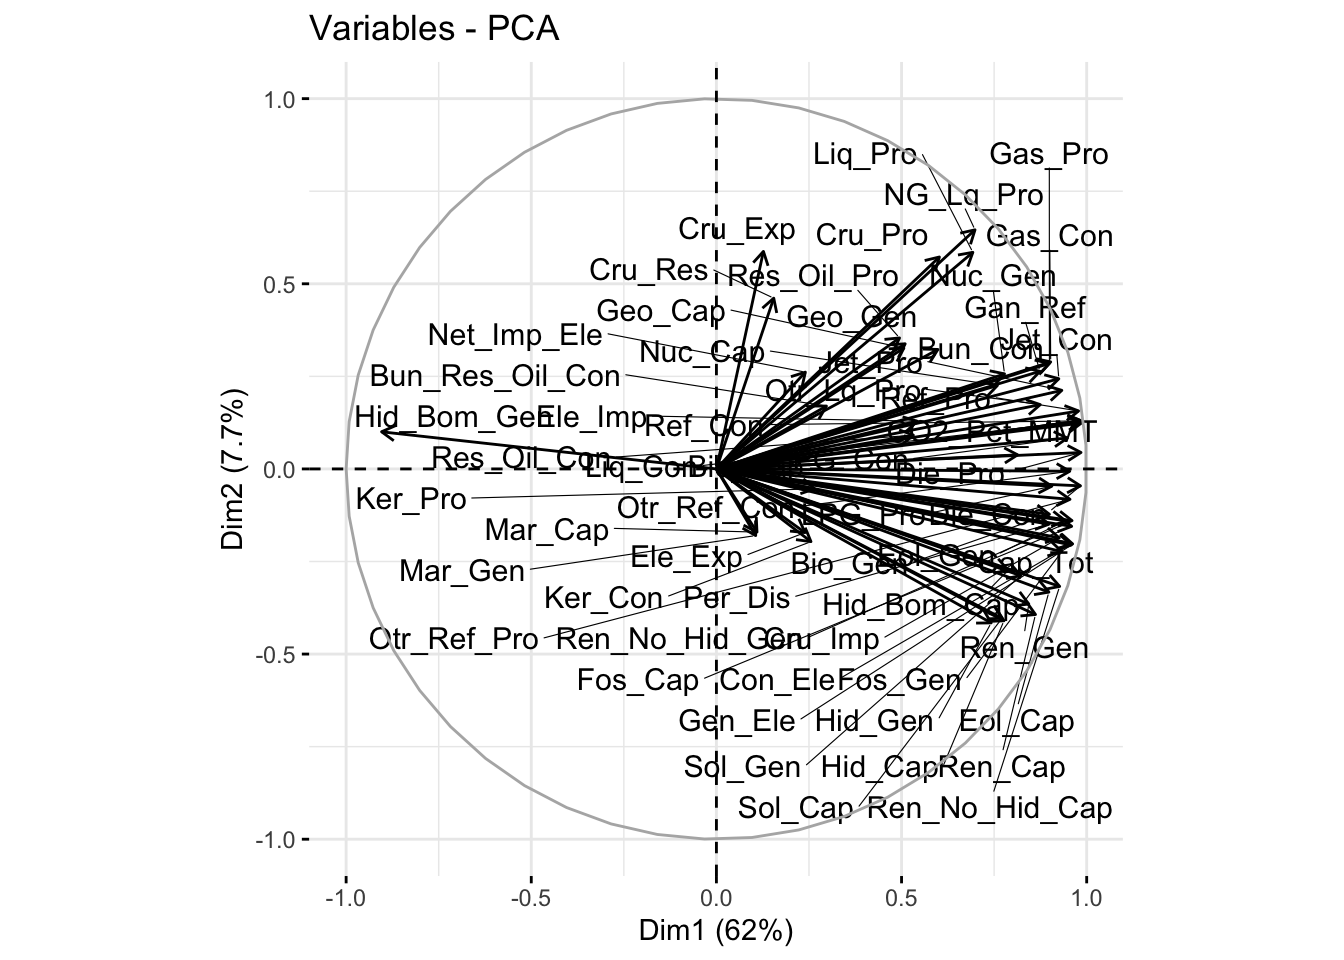
\includegraphics{T02_AEDatos_files/figure-latex/preg_05a-1.pdf}

Por esto se procede a graficar únicamente las 30 variables que más
aportan a los datos como se aconseja en la sección de ayuda, mediante
\texttt{fviz\_pca\_var(acp\_c,axes=c(1,2),repel=TRUE,select.var\ =\ list(contrib\ =\ 30))}
obteniendo la siguiente grafica, de esta podemos concluir que dimension
1 o PCA 1, agrupa el 62\% de los datos y el PCA 2 el 7,7\%, siendo
necesario apoyarnos en mas PCAs para lograr tomar un 80\% de los datos y
tener una mejor representacion de los datos de las 57 variables. Por
otro lado, las flechas asignadas para cada variable indican la
contribución en cada PCA, dando como resultado que en su mayoria aportan
a la dimension 1 con una longitud muy parecida o agrupada entre cada
variable dado que eliminamos las que menos contribuían, teniendo 2 casos
visiblemente diferentes como lo son las variables Hid\_Bom\_Gen (
Hydroelectric\_pumped\_storage\_electricity\_net\_generation\_BKWH), la
cual se ubica en el cuadrante 2 aportanto al PCA1 negativo, y la
variable NG\_Lq\_Pro (Natural\_gas\_plant\_liquids\_production\_TBPD),
la cual aporta en la dimension 1 y 2.

En contraste al ejercicio de clase, en este contamos con una cantidad
mayor de componentes relevantes para el análisis, por lo cual, realice
el mismo gráfico anterior pero ahora sobre el plano factorial conformado
por los componentes 2 y 3. ¿Qué conclusiones podemos sacar de este
gráfico?

Utilizando la linea de codigo
\texttt{fviz\_pca\_var(acp\_c,\ axes\ =\ c(2,\ 3),repel=TRUE,select.var\ =\ list(contrib\ =\ 30))},
Los datos de las variables en estos componentes tienen una menor
contribución y estos se puede evidenciar en la magnitud de las flechas,
junto a esto, se puede ver que hay una mayor distribución en los
diferentes cuadrantes del diagrama fasorial, es importante resaltar como
el PCA3 tiene 7\% de los datos, con estos 3 PCAs agruparíamos el 76.7\%
de los datos, sería necesario tomar más componentes principales para
llegar al 80\%, lo cual nos daría una representación objetiva de los
datos.

\begin{Shaded}
\begin{Highlighting}[]
\FunctionTok{fviz\_pca\_var}\NormalTok{(acp\_c, }\AttributeTok{axes =} \FunctionTok{c}\NormalTok{(}\DecValTok{2}\NormalTok{, }\DecValTok{3}\NormalTok{),}\AttributeTok{repel=}\ConstantTok{TRUE}\NormalTok{,}\AttributeTok{select.var =} \FunctionTok{list}\NormalTok{(}\AttributeTok{contrib =} \DecValTok{30}\NormalTok{))}
\end{Highlighting}
\end{Shaded}

\includegraphics{T02_AEDatos_files/figure-latex/preg_05c-1.pdf}

\subsubsection{Pregunta 6}\label{pregunta-6}

\(w_6=10\)\\
Ahora examine con detenimiento el mapa de individuos sobre los planos
factoriales que conforman las componentes (1,2) y (2,3). ¿Qué
conclusiones puede sacar según la cercanía de algunas UE?

\begin{Shaded}
\begin{Highlighting}[]
\NormalTok{res.pca }\OtherTok{\textless{}{-}} \FunctionTok{PCA}\NormalTok{(datos[,}\SpecialCharTok{{-}}\DecValTok{1}\NormalTok{], }\AttributeTok{graph =} \ConstantTok{FALSE}\NormalTok{)}
\FunctionTok{fviz\_pca\_ind}\NormalTok{(res.pca, }\AttributeTok{geom.ind =} \StringTok{"point"}\NormalTok{, }
             \AttributeTok{col.ind =} \StringTok{"\#FC4E07"}\NormalTok{, }
             \AttributeTok{axes =} \FunctionTok{c}\NormalTok{(}\DecValTok{1}\NormalTok{, }\DecValTok{2}\NormalTok{), }
             \AttributeTok{pointsize =} \FloatTok{1.5}\NormalTok{) }
\end{Highlighting}
\end{Shaded}

\includegraphics{T02_AEDatos_files/figure-latex/unnamed-chunk-13-1.pdf}
Dim1 (62\%):

\begin{itemize}
\item
  Este eje captura la mayor parte de la variabilidad, sugiriendo que una
  única dimensión ordena eficientemente a los países.
\item
  Rango de valores: Los países se distribuyen desde -10 (extremo
  izquierdo) hasta 40 (extremo derecho), indicando una fuerte
  polarización.
\end{itemize}

Dim2 (7.7\%):

\begin{itemize}
\tightlist
\item
  Su contribución parece marginal, por lo que el análisis se centra en
  Dim1 (62\%).
\end{itemize}

Distribución de Países

Patrón de dispersión:

\begin{itemize}
\item
  Extremo derecho: Países con características inusuales.
\item
  Centro (valores cercanos a 0): Países con perfiles energéticos
  similares.
\item
  Extremo izquierdo (valores negativos): Países con patrones atípicos.
\end{itemize}

\begin{Shaded}
\begin{Highlighting}[]
\FunctionTok{fviz\_pca\_ind}\NormalTok{(res.pca, }\AttributeTok{geom.ind =} \StringTok{"point"}\NormalTok{, }
             \AttributeTok{col.ind =} \StringTok{"blue"}\NormalTok{, }
             \AttributeTok{axes =} \FunctionTok{c}\NormalTok{(}\DecValTok{2}\NormalTok{, }\DecValTok{3}\NormalTok{), }
             \AttributeTok{pointsize =} \FloatTok{1.5}\NormalTok{) }
\end{Highlighting}
\end{Shaded}

\includegraphics{T02_AEDatos_files/figure-latex/unnamed-chunk-14-1.pdf}
Dim3 (7\%) y Dim2 (7.7\%):

Ambos componentes explican una proporción baja de varianza total (14.7\%
combinada). Esto sugiere que:

\begin{itemize}
\tightlist
\item
  La estructura subyacente de los datos es alta-dimensional (muchas
  variables influyentes no capturadas en estos ejes).
\end{itemize}

Distribución de Países

\begin{itemize}
\item
  Los puntos (países) están dispersos en un rango de -10 a 10 en ambos
  ejes, sin agrupamientos claros. Esto indica:
\item
  No hay perfiles dominantes que agrupen a múltiples países.
\item
  Outliers potenciales: Países en extremos (ej., cerca de (-10, 10))
  podrían ser casos atípicos.
\end{itemize}

\subsubsection{Pregunta 7}\label{pregunta-7}

\(w_7=10\)\\
Como hemos observado en clase, el ACP es una técnica bastante sensible a
datos atípicos, ejecute nuevamente el ACP retirando del conjunto de
datos a Estados Unidos, China, Arabia Saudi y Rusia. ¿En que cambia el
ACP al excluir estos países?. ¿Se perciben clusters de países con mayor
claridad?. Calcule únicamente el ACP normado.

\begin{Shaded}
\begin{Highlighting}[]
\CommentTok{\#se retiran los países propuestos}
\NormalTok{retirados }\OtherTok{\textless{}{-}} \FunctionTok{c}\NormalTok{(}\StringTok{"UnitedStates"}\NormalTok{, }\StringTok{"China"}\NormalTok{, }\StringTok{"SaudiArabia"}\NormalTok{, }\StringTok{"Russia"}\NormalTok{)}
 
\CommentTok{\#creación de la nueva tabla de datos que ya no tienen los países retirados}
\NormalTok{paises\_filtrados }\OtherTok{\textless{}{-}}\NormalTok{ datos[}\SpecialCharTok{!}\NormalTok{datos}\SpecialCharTok{$}\NormalTok{Country }\SpecialCharTok{\%in\%}\NormalTok{ retirados, ]}
\NormalTok{columnas\_numericas }\OtherTok{\textless{}{-}} \FunctionTok{names}\NormalTok{(paises\_filtrados)[}\SpecialCharTok{{-}}\DecValTok{1}\NormalTok{]}
 
\NormalTok{pca\_normalizado }\OtherTok{\textless{}{-}} \FunctionTok{prcomp}\NormalTok{(paises\_filtrados[, columnas\_numericas], }\AttributeTok{center =} \ConstantTok{TRUE}\NormalTok{, }\AttributeTok{scale =} \ConstantTok{TRUE}\NormalTok{)}
\NormalTok{pca\_sin\_normalizar }\OtherTok{\textless{}{-}} \FunctionTok{prcomp}\NormalTok{(paises\_filtrados[, columnas\_numericas], }\AttributeTok{center =} \ConstantTok{FALSE}\NormalTok{, }\AttributeTok{scale =} \ConstantTok{FALSE}\NormalTok{)}
 
\NormalTok{contribucion\_normalizado }\OtherTok{\textless{}{-}}\NormalTok{ pca\_normalizado}\SpecialCharTok{$}\NormalTok{sdev}\SpecialCharTok{\^{}}\DecValTok{2}
\NormalTok{contribucion\_sin\_normalizar }\OtherTok{\textless{}{-}}\NormalTok{ pca\_sin\_normalizar}\SpecialCharTok{$}\NormalTok{sdev}\SpecialCharTok{\^{}}\DecValTok{2}

\NormalTok{contribuciones\_df }\OtherTok{\textless{}{-}} \FunctionTok{data.frame}\NormalTok{(}
  \AttributeTok{Contribucion\_Normalizado =}\NormalTok{ contribucion\_normalizado,}
  \AttributeTok{Contribucion\_Sin\_Normalizar =}\NormalTok{ contribucion\_sin\_normalizar}
\NormalTok{)}
 
\NormalTok{varianza\_explicada }\OtherTok{\textless{}{-}}\NormalTok{ pca\_normalizado}\SpecialCharTok{$}\NormalTok{sdev}\SpecialCharTok{\^{}}\DecValTok{2}
 
\NormalTok{varianza\_acumulada }\OtherTok{\textless{}{-}} \FunctionTok{cumsum}\NormalTok{(varianza\_explicada) }\SpecialCharTok{/} \FunctionTok{sum}\NormalTok{(varianza\_explicada)}
 
\FunctionTok{head}\NormalTok{(contribuciones\_df, }\AttributeTok{n=}\DecValTok{10}\NormalTok{)}
\end{Highlighting}
\end{Shaded}

\begin{verbatim}
##    Contribucion_Normalizado Contribucion_Sin_Normalizar
## 1                27.8996281                 4098283.841
## 2                 5.8387300                 1445037.166
## 3                 4.6204396                   86544.805
## 4                 3.7753312                   41993.071
## 5                 2.8210627                   26544.386
## 6                 2.2286043                   14081.658
## 7                 2.0557117                   10294.495
## 8                 1.6001717                    8629.487
## 9                 1.3866329                    5178.434
## 10                0.8667378                    3747.178
\end{verbatim}

Los países retirados presentan datos atípicos ya que son grandes
consumidores de recursos energéticos como la electricidad o el petróleo
y por otra parte, también se tienen grandes productores de aquellos
recursos.

Las variaciones de las contribuciones de los datos normalizados si se
comparan con los primeros resultados cuando estaban todos los países,
muestran menos saltos, de manera similar sucede con los datos sin
normalizar.

Lo anterior debido a que los países retirados presentaban datos altos si
se comparaban con otros, lo que hacía que la escala de datos fuera mucho
mayor. Al ser retirados estos países con datos atípicos, contribuye a
buscar más eficazmente países con comportamientos más comunes entre sí y
permite sean agrupados de o subdivididos de manera geográfica, por
ejemplo.

\subsection{Clustering}\label{clustering}

\begin{center}\rule{0.5\linewidth}{0.5pt}\end{center}

Los puntos 8 a 11 se realizarán excluyendo de la base de datos los
países atípicos mencionados en el punto 7 (es decir, retirando
`UnitedStates',`China',`SaudiArabia',`Russia').

\subsubsection{Pregunta 8}\label{pregunta-8}

\(w_8=8\)\\
De acuerdo a lo aprendido en la clase de agrupamiento, utilice el primer
plano factorial para determinar de manera aproximada el número de grupos
en el análisis. ¿Cuántos clusters espera que existan en el conjunto de
datos?

\begin{Shaded}
\begin{Highlighting}[]
\NormalTok{PrimerasComponentes }\OtherTok{\textless{}{-}}\NormalTok{ pca\_normalizado}\SpecialCharTok{$}\NormalTok{x[, }\FunctionTok{c}\NormalTok{(}\DecValTok{1}\NormalTok{, }\DecValTok{2}\NormalTok{)] }\CommentTok{\#Seleccion de la ubicación de cada país en las dos componentes principales}
\NormalTok{distancia\_total }\OtherTok{\textless{}{-}} \FunctionTok{numeric}\NormalTok{(}\DecValTok{10}\NormalTok{)  }\CommentTok{\# Crear vector de longitud 10}

\ControlFlowTok{for}\NormalTok{ (i }\ControlFlowTok{in} \DecValTok{1}\SpecialCharTok{:}\DecValTok{10}\NormalTok{) }
\NormalTok{  \{}
\NormalTok{    kmeans\_model }\OtherTok{\textless{}{-}} \FunctionTok{kmeans}\NormalTok{(PrimerasComponentes, }\AttributeTok{centers =}\NormalTok{ i) }\CommentTok{\#agrupar los datos ubicados en el plano en i cantidad de grupos}
\NormalTok{    distancia\_total[i] }\OtherTok{\textless{}{-}}\NormalTok{ kmeans\_model}\SpecialCharTok{$}\NormalTok{tot.withinss }\CommentTok{\#sumar la distancia total de la agrupación i}
\NormalTok{  \} }
  \FunctionTok{plot}\NormalTok{(}\DecValTok{1}\SpecialCharTok{:}\DecValTok{10}\NormalTok{,distancia\_total,}\AttributeTok{ylab=}\StringTok{"Distancia por número de grupos"}\NormalTok{, }\AttributeTok{xlab =} \StringTok{\textquotesingle{}1:10\textquotesingle{}}\NormalTok{, }\AttributeTok{type=}\StringTok{\textquotesingle{}b\textquotesingle{}}\NormalTok{)}
\end{Highlighting}
\end{Shaded}

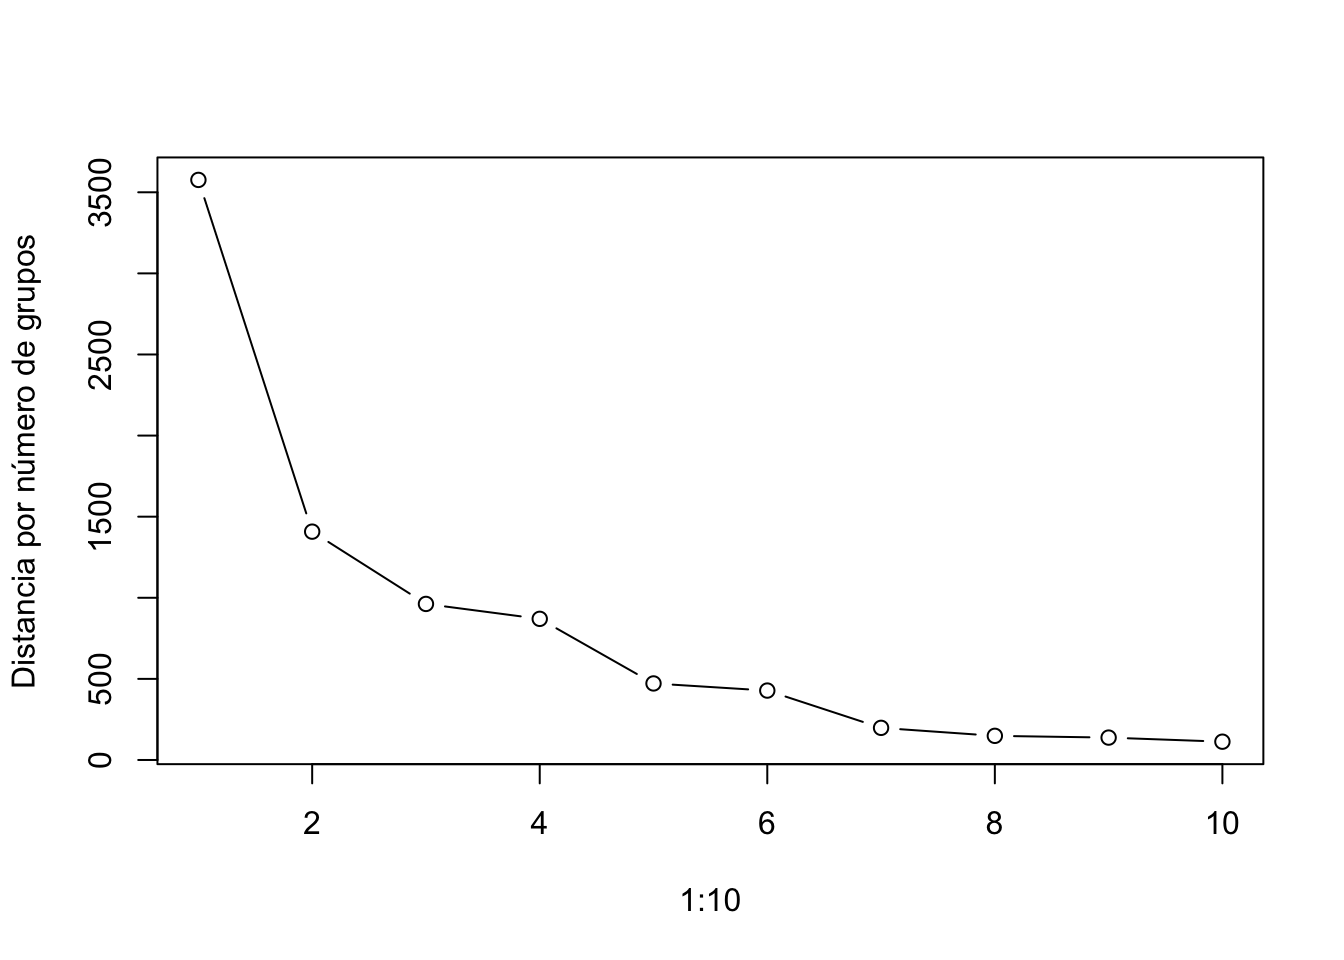
\includegraphics{T02_AEDatos_files/figure-latex/preg_08-1.pdf}

De acuerdo con la imagen anterior, se pueden esperar 4 clústeres o
grupos ya que con esta cantidad se obtiene una reducción de distancia
significativa y con cantidades mayores las reducciones son pequeñas.

\subsubsection{Pregunta 9}\label{pregunta-9}

\(w_9=12\)\\
Mediante el método de reducción de varianza explicada, determine un
número fijo de clusters para su análisis. No tiene que ser el mismo
número que el elegido por su compañero, recuerde que ninguno conoce las
etiquetas reales de los grupos de los países.

Respecto de la curva de codo de obtenida en el punto anterior, se
considera que un numero ideal de clusters para analisis es k=4, dado
que, luego de este, la disminucion se reduce significativamente la mejor
en valores superiores de k no es representativa

\begin{Shaded}
\begin{Highlighting}[]
\CommentTok{\#PrimerasComponentes \textless{}{-} pca\_normalizado$x[, c(1, 2)] \#Seleccion de la ubicación de cada país en las dos componentes principales}
\NormalTok{distancia\_total }\OtherTok{\textless{}{-}} \FunctionTok{numeric}\NormalTok{(}\DecValTok{4}\NormalTok{)  }\CommentTok{\# Crear vector de longitud 10}
\ControlFlowTok{for}\NormalTok{ (i }\ControlFlowTok{in} \DecValTok{1}\SpecialCharTok{:}\DecValTok{4}\NormalTok{) }
\NormalTok{  \{}
\NormalTok{    kmeans\_model }\OtherTok{\textless{}{-}} \FunctionTok{kmeans}\NormalTok{(PrimerasComponentes, }\AttributeTok{centers =}\NormalTok{ i) }\CommentTok{\#agrupar los datos ubicados en el plano en i cantidad de grupos}
\NormalTok{    distancia\_total[i] }\OtherTok{\textless{}{-}}\NormalTok{ kmeans\_model}\SpecialCharTok{$}\NormalTok{tot.withinss }\CommentTok{\#sumar la distancia total de la agrupación i}
\NormalTok{  \} }
  \FunctionTok{plot}\NormalTok{(}\DecValTok{1}\SpecialCharTok{:}\DecValTok{4}\NormalTok{,distancia\_total,}\AttributeTok{ylab=}\StringTok{"Distancia por número de grupos"}\NormalTok{, }\AttributeTok{xlab =} \StringTok{\textquotesingle{}1:4\textquotesingle{}}\NormalTok{, }\AttributeTok{type=}\StringTok{\textquotesingle{}b\textquotesingle{}}\NormalTok{)}
\end{Highlighting}
\end{Shaded}

\includegraphics{T02_AEDatos_files/figure-latex/preg_09-1.pdf}

\subsubsection{Pregunta 10}\label{pregunta-10}

\(w_{10}=12\)\\
Determine mediante k-means y aglomeración jerárquica (usando enlace
promedio) la clasificación en grupos para los países de estudio.
Considere todas las variables de estudio ¿son diferentes los resultados
de los dos análisis cluster?

\begin{Shaded}
\begin{Highlighting}[]
\FunctionTok{set.seed}\NormalTok{(}\DecValTok{100}\NormalTok{)}
\NormalTok{kmeans\_m }\OtherTok{\textless{}{-}} \FunctionTok{kmeans}\NormalTok{(pca\_normalizado}\SpecialCharTok{$}\NormalTok{x, }\AttributeTok{centers =} \DecValTok{4}\NormalTok{)}\CommentTok{\# aplicar K{-}means con 4 clusters}
\NormalTok{clusters }\OtherTok{\textless{}{-}}\NormalTok{ kmeans\_m}\SpecialCharTok{$}\NormalTok{cluster }

 \CommentTok{\# mostrar tabla con los 4 clusters}
 \FunctionTok{table}\NormalTok{(clusters)}
\end{Highlighting}
\end{Shaded}

\begin{verbatim}
## clusters
##  1  2  3  4 
##  8 10  2 87
\end{verbatim}

\begin{Shaded}
\begin{Highlighting}[]
\CommentTok{\# aplicar metodo de aglomeracion promedio}
\NormalTok{d\_aglomerados }\OtherTok{\textless{}{-}} \FunctionTok{hclust}\NormalTok{(}\FunctionTok{dist}\NormalTok{(pca\_normalizado}\SpecialCharTok{$}\NormalTok{x), }\AttributeTok{method =} \StringTok{"average"}\NormalTok{)}

\CommentTok{\#lleva el arbol jerarquico a 4 grupos para poder comparar con el resultado de kmeans}
\NormalTok{clusters\_aglomerados }\OtherTok{\textless{}{-}} \FunctionTok{cutree}\NormalTok{(d\_aglomerados, }\AttributeTok{k =} \DecValTok{4}\NormalTok{) }

\CommentTok{\#resultados de de los 4 grupos aglomerados}
\FunctionTok{table}\NormalTok{(clusters\_aglomerados) }
\end{Highlighting}
\end{Shaded}

\begin{verbatim}
## clusters_aglomerados
##   1   2   3   4 
## 101   2   2   2
\end{verbatim}

Si, Son diferentes los resultados entre k-means y aglomeración
jerárquica promedio, podemos observar en los resultados que en el caso
de K-means el cluster 3 contiene 87 paises, y en el caso de agrupamiento
promedio, el grupo 3 contiene 2 paises. El agrupamiento jerarquico
promedio agrupa 101 países en el grupo 1, como se vio en clase, los
diferentes métodos de agrupamiento (clusters) difieren al momento de
tomar las distancias entre los diferentes valores para irlos agrupando,
lo cual queda demostrado en la comparación de los resultados anteriores.

\subsubsection{Pregunta 11}\label{pregunta-11}

\(w_{11}=12\)\\
Grafique mediante boxplot la distribución de las 5 variables
seleccionadas en el punto 2 diferenciando por los grupos encontrados
mediante k-means (es decir, obtenga un boxplot por variable y por grupo:
si por ejemplo k-means indica un total de 3 grupos, realice 3 boxplots,
uno por grupo, para cada una de las 5 variables). ¿Observa diferencias
importantes entre las distribuciones por grupos de la misma variable?

\begin{Shaded}
\begin{Highlighting}[]
\NormalTok{Variables\_Escogidas }\OtherTok{=}\NormalTok{ paises\_filtrados[, }\FunctionTok{c}\NormalTok{(}\StringTok{"Country"}\NormalTok{ ,}\StringTok{"Refined\_petroleum\_products\_consumption\_TBPD"}\NormalTok{, }\StringTok{"Refined\_petroleum\_products\_production\_TBPD"}\NormalTok{, }\StringTok{"Electricity\_exports\_BKWH"}\NormalTok{, }\StringTok{"Electricity\_imports\_BKWH"}\NormalTok{, }\StringTok{"Electricity\_installed\_capacity\_MK"}\NormalTok{)]}
\NormalTok{Variables\_Escogidas}\SpecialCharTok{$}\NormalTok{Grupo }\OtherTok{\textless{}{-}}\NormalTok{ clusters }\CommentTok{\# agregar al set de datos una columna con el grupo}

\CommentTok{\# boxplot de Refined\_petroleum\_products\_consumption\_TBPD}
\FunctionTok{ggplot}\NormalTok{(Variables\_Escogidas, }\FunctionTok{aes}\NormalTok{(}\AttributeTok{x =} \FunctionTok{factor}\NormalTok{(Grupo), }\AttributeTok{y =}\NormalTok{ Refined\_petroleum\_products\_consumption\_TBPD)) }\SpecialCharTok{+}
  \FunctionTok{geom\_boxplot}\NormalTok{() }\SpecialCharTok{+}
  \FunctionTok{theme\_minimal}\NormalTok{() }\SpecialCharTok{+}
  \FunctionTok{labs}\NormalTok{(}
    \AttributeTok{title =} \StringTok{"Consumo de derivados de petróleo por grupo"}\NormalTok{,}
    \AttributeTok{x =} \StringTok{"Grupo"}\NormalTok{,}
    \AttributeTok{y =} \StringTok{"Consumo (TBPD)"}\NormalTok{ )}
\end{Highlighting}
\end{Shaded}

\includegraphics{T02_AEDatos_files/figure-latex/preg_11a-1.pdf}

\begin{Shaded}
\begin{Highlighting}[]
\CommentTok{\# boxplot de Refined\_petroleum\_products\_production\_TBPD}
\FunctionTok{ggplot}\NormalTok{(Variables\_Escogidas, }\FunctionTok{aes}\NormalTok{(}\AttributeTok{x =} \FunctionTok{factor}\NormalTok{(Grupo), }\AttributeTok{y =}\NormalTok{ Refined\_petroleum\_products\_production\_TBPD)) }\SpecialCharTok{+}
  \FunctionTok{geom\_boxplot}\NormalTok{() }\SpecialCharTok{+}
  \FunctionTok{theme\_minimal}\NormalTok{() }\SpecialCharTok{+}
  \FunctionTok{labs}\NormalTok{(}
    \AttributeTok{title =} \StringTok{"Producción de derivados de petróleo por grupo"}\NormalTok{,}
    \AttributeTok{x =} \StringTok{"Grupo"}\NormalTok{,}
    \AttributeTok{y =} \StringTok{"Producción (TBPD)"}\NormalTok{ )}
\end{Highlighting}
\end{Shaded}

\includegraphics{T02_AEDatos_files/figure-latex/preg_11a-2.pdf}

\begin{Shaded}
\begin{Highlighting}[]
\CommentTok{\# boxplot de Electricity\_exports\_BKWH}
\FunctionTok{ggplot}\NormalTok{(Variables\_Escogidas, }\FunctionTok{aes}\NormalTok{(}\AttributeTok{x =} \FunctionTok{factor}\NormalTok{(Grupo), }\AttributeTok{y =}\NormalTok{ Electricity\_exports\_BKWH)) }\SpecialCharTok{+}
  \FunctionTok{geom\_boxplot}\NormalTok{() }\SpecialCharTok{+}
  \FunctionTok{theme\_minimal}\NormalTok{() }\SpecialCharTok{+}
  \FunctionTok{labs}\NormalTok{(}
    \AttributeTok{title =} \StringTok{"Exportaciones de electricidad"}\NormalTok{,}
    \AttributeTok{x =} \StringTok{"Grupo"}\NormalTok{,}
    \AttributeTok{y =} \StringTok{"Exportación (BKWH)"}\NormalTok{)}
\end{Highlighting}
\end{Shaded}

\includegraphics{T02_AEDatos_files/figure-latex/preg_11a-3.pdf}

\begin{Shaded}
\begin{Highlighting}[]
\CommentTok{\# boxplot de Electricity\_imports\_BKWH}
\FunctionTok{ggplot}\NormalTok{(Variables\_Escogidas, }\FunctionTok{aes}\NormalTok{(}\AttributeTok{x =} \FunctionTok{factor}\NormalTok{(Grupo), }\AttributeTok{y =}\NormalTok{ Electricity\_imports\_BKWH)) }\SpecialCharTok{+}
  \FunctionTok{geom\_boxplot}\NormalTok{() }\SpecialCharTok{+}
  \FunctionTok{theme\_minimal}\NormalTok{() }\SpecialCharTok{+}
  \FunctionTok{labs}\NormalTok{(}
    \AttributeTok{title =} \StringTok{"Importaciones de electricidad"}\NormalTok{,}
    \AttributeTok{x =} \StringTok{"Grupo"}\NormalTok{,}
    \AttributeTok{y =} \StringTok{"Importación (BKWH)"}\NormalTok{)}
\end{Highlighting}
\end{Shaded}

\includegraphics{T02_AEDatos_files/figure-latex/preg_11a-4.pdf}

\begin{Shaded}
\begin{Highlighting}[]
\CommentTok{\# boxplot de Electricity\_installed\_capacity\_MK}
\FunctionTok{ggplot}\NormalTok{(Variables\_Escogidas, }\FunctionTok{aes}\NormalTok{(}\AttributeTok{x =} \FunctionTok{factor}\NormalTok{(Grupo), }\AttributeTok{y =}\NormalTok{ Electricity\_installed\_capacity\_MK)) }\SpecialCharTok{+}
  \FunctionTok{geom\_boxplot}\NormalTok{() }\SpecialCharTok{+}
  \FunctionTok{theme\_minimal}\NormalTok{() }\SpecialCharTok{+}
  \FunctionTok{labs}\NormalTok{(}
    \AttributeTok{title =} \StringTok{"Capacidad instalada"}\NormalTok{,}
    \AttributeTok{x =} \StringTok{"Grupo"}\NormalTok{,}
    \AttributeTok{y =} \StringTok{"Capacidad instalada (MK)"}\NormalTok{)}
\end{Highlighting}
\end{Shaded}

\includegraphics{T02_AEDatos_files/figure-latex/preg_11a-5.pdf}

\subsection{Referencias}\label{referencias}

\begin{enumerate}
\def\labelenumi{\arabic{enumi}.}
\tightlist
\item
  \href{https://rmarkdown.rstudio.com/articles_intro.html}{Introduction
  to R markdown}
\item
  MarkDown Guide -
  \href{https://www.markdownguide.org/basic-syntax/}{Basic Syntax}
\item
  \href{https://github.com/rstudio/cheatsheets/blob/main/data-visualization.pdf}{Data
  Visualization CheatSheet}
\item
  \href{https://github.com/aosoriom7/MER_AED_2025I}{Repositorio} del
  Taller en Github
\item
  \href{https://aosoriom7.github.io/MER_AED_2025I/scripts/02.html}{Pagina}
  web del taller en Gihub Pages
\end{enumerate}

\end{document}
